
\documentclass{sig-alternate-05-2015}

\usepackage[ruled, commentsnumbered, longend]{algorithm2e}

\begin{document}

% Copyright
\setcopyright{acmcopyright}
%\setcopyright{acmlicensed}
%\setcopyright{rightsretained}
%\setcopyright{usgov}
%\setcopyright{usgovmixed}
%\setcopyright{cagov}
%\setcopyright{cagovmixed}


% DOI
%%\doi{10.475/123_4}

% ISBN
%%\isbn{123-4567-24-567/08/06}

%Conference
\conferenceinfo{KDD '16}{August 13--17, 2016, San Fransisco, CA, USA}

\acmPrice{\$15.00}

%
% --- Author Metadata here ---
%\CopyrightYear{2007} % Allows default copyright year (20XX) to be over-ridden - IF NEED BE.
%\crdata{0-12345-67-8/90/01}  % Allows default copyright data (0-89791-88-6/97/05) to be over-ridden - IF NEED BE.
% --- End of Author Metadata ---


\title{Multi-Stage Ensemble and Feature Engineering for MOOC Dropout Prediction}
\numberofauthors{9}
\author{
%%
%% Let's clean up the author section so that it looks more concise.
%%
\alignauthor Jeong-Yoon Lee \\
       \affaddr{Conversion Logic}\\
%%       \affaddr{\small 12300 Wilshire Blvd. Los Angeles, CA 90025, USA}\\
       \email{\small jeong@conversionlogic.com}
\alignauthor Andreas Toescher\\
       \affaddr{Opera Solutions}\\
%%       \affaddr{\small Hauptplatz 12, 8580 Koeflach, Austria}\\
       \email{\small andreas.toescher@commendo.at}
\alignauthor Kohei Ozaki\\
       \affaddr{Recruit Technologies}\\
%%       \affaddr{\small Kamiyacho MT Bldg 18F, 4-3-20 Toranomon, Minato-ku, Tokyo 105-0001, Japan}\\
       \email{ \small kohei\_ozaki@r.recruit.co.jp}
\and
\alignauthor Mert Bay\\
       \affaddr{Conversion Logic}\\
%%       \affaddr{\small 12300 Wilshire Blvd. Los Angeles, CA 90025, USA}\\
       \email{\small mert@conversionlogic.com}
\alignauthor Michael Jahrer\\
       \affaddr{Opera Solutions}\\
%%       \affaddr{\small Hauptplatz 12, 8580 Koeflach, Austria}\\
       \email{\small michael.jahrer@commendo.at}
\alignauthor Tam T. Nguyen\\
       \affaddr{Institute for Infocomm Research}\\
%%       \affaddr{\small 1 Fusionopolis Way, \#21-01 Connexis, Singapore 138632}\\
       \email{\small nguyentt@i2r.a-star.edu.sg}
}
% There's nothing stopping you putting the seventh, eighth, etc.
% author on the opening page (as the 'third row') but we ask,
% for aesthetic reasons that you place these 'additional authors'
% in the \additional authors block, viz.
\additionalauthors{Additional authors: Xiaocong Zhou (Tsinghua University,
email: {\texttt{infinitezxc@gmail.com}}), Song Chen (AIG, email: {\texttt{song.chen@aig.com}}) and Peng Yan
(NetEase Youdao, email: {\texttt{yanpeng@rd.netease.com}}).}

\date{9 February 2016}
\maketitle
\begin{abstract}
In this paper, we present the winning solution of KDD Cup 2015, where participants are asked to predict dropouts in a Massive Open Online Course (MOOC) platform.  
Our approach demonstrates best practices in feature engineering dealing with complex real world data, and pushes forward the state-of-the-art ensemble technique.
We began with feature engineering and extracted XXX and YYY features from raw student activity logs, course enrollment, and course material data.  
Then, we trained 64 classifiers with 8 different algorithms and different subsets of extracted features.  Lastly, we blended predictions of classifiers with the multi-stage ensemble framework.  
Our final solution achieved AUC scores of 0.90918 and 0.90744 on the public and private leaderboards respectively, and put us to the 1st place out of 821 teams.
% 7 algorithms: GBDT, NN/DAE+NN, LR, FFM/FM, ET, KRR, Boosting of Linear Regressor, 
\end{abstract}

%
% The code below should be generated by the tool at
% http://dl.acm.org/ccs.cfm
% Please copy and paste the code instead of the example below. 
%
\begin{CCSXML}
<ccs2012>
<concept>
<concept_id>10010147.10010257.10010258.10010259.10010263</concept_id>
<concept_desc>Computing methodologies~Supervised learning by classification</concept_desc>
<concept_significance>500</concept_significance>
</concept>
<concept>
<concept_id>10010147.10010257.10010321.10010333</concept_id>
<concept_desc>Computing methodologies~Ensemble methods</concept_desc>
<concept_significance>500</concept_significance>
</concept>
<concept>
<concept_id>10010147.10010257.10010339</concept_id>
<concept_desc>Computing methodologies~Cross-validation</concept_desc>
<concept_significance>300</concept_significance>
</concept>
</ccs2012>
\end{CCSXML}

\ccsdesc[500]{Computing methodologies~Supervised learning by classification}
\ccsdesc[500]{Computing methodologies~Ensemble methods}
\ccsdesc[300]{Computing methodologies~Cross-validation}

%
% End generated code
%

%
%  Use this command to print the description
%
\printccsdesc


\keywords{KDD Cup, Feature Engineering, Ensemble Learning}

\section{Introduction}
The task of KDD Cup 2015 is to predict the likelihood of dropout for students on XuetangX, one of the largest Massive Open Online Course (MOOC) platforms in China.

Activity logs of 200,906 enrollments from 112,448 students across 39 courses are provided.
Each activity is described by 6 fields of the username, course ID, timestamp, source, event, and object. 
For each object, 3 additional fields of the category, children, and start date are provided.
The training set consists of 8,157,278 logs from 120,543 enrollments with the target variable indicating if a student dropped out.  
The test set consists of 5,387,848 logs from 80,363 enrollments.
The full description of the data sets is available in \cite{kddcup2015_data}



Our final solution is a joint work from 9 data scientists, distributed around the world.
The pipeline from raw data to final solution is as follows:
\begin{itemize}
  \setlength\itemsep{0em}
  \item Hand crafted feature engineering (most of hard work)
  \item Automatic feature design (autoencoder)
  \item Individual models (gbm, nn, factor model,..)
  \item Stage-I ensemble (blends individual models)
  \item Stage-II ensemble (blends stage-I ensemble models)
  \item Stage-III ensemble (blends stage-II ensemble models)
\end{itemize}

% I think our ensemble framework is different from Otto competition winner's:  Theirs is a stage-II and ours is a stage-III.
% This approach was published by a winning team of Otto kaggle competition \cite{otto},\cite{triskelion}.
\section{Feature Engineering}
Our team members extracted 7 feature sets, namely F1, F2, F3, F4, F5, F6, and F7 from raw data independently.

\subsection{Data Sets}
Activity logs of 200,906 enrollments from 112,448 students across 39 courses are provided.
Each activity is described by 6 fields of the username, course ID, timestamp, source, event, and object. 
For each object, 3 additional fields of the category, children, and start date are provided.
The training set consists of 8,157,278 logs from 120,543 enrollments with the target variable indicating if a student dropped out.  
The test set consists of 5,387,848 logs from 80,363 enrollments.
The full description of the data sets is available in \cite{kddcup2015_data}. In general, this data can be organized in three dimension space, object, time, and event as shown in Figure~\ref{fig:cube}. Feature engineering tasks were carried out based on these views.

\begin{figure*}[!t]
	\caption{Data Cube}
	\centering
	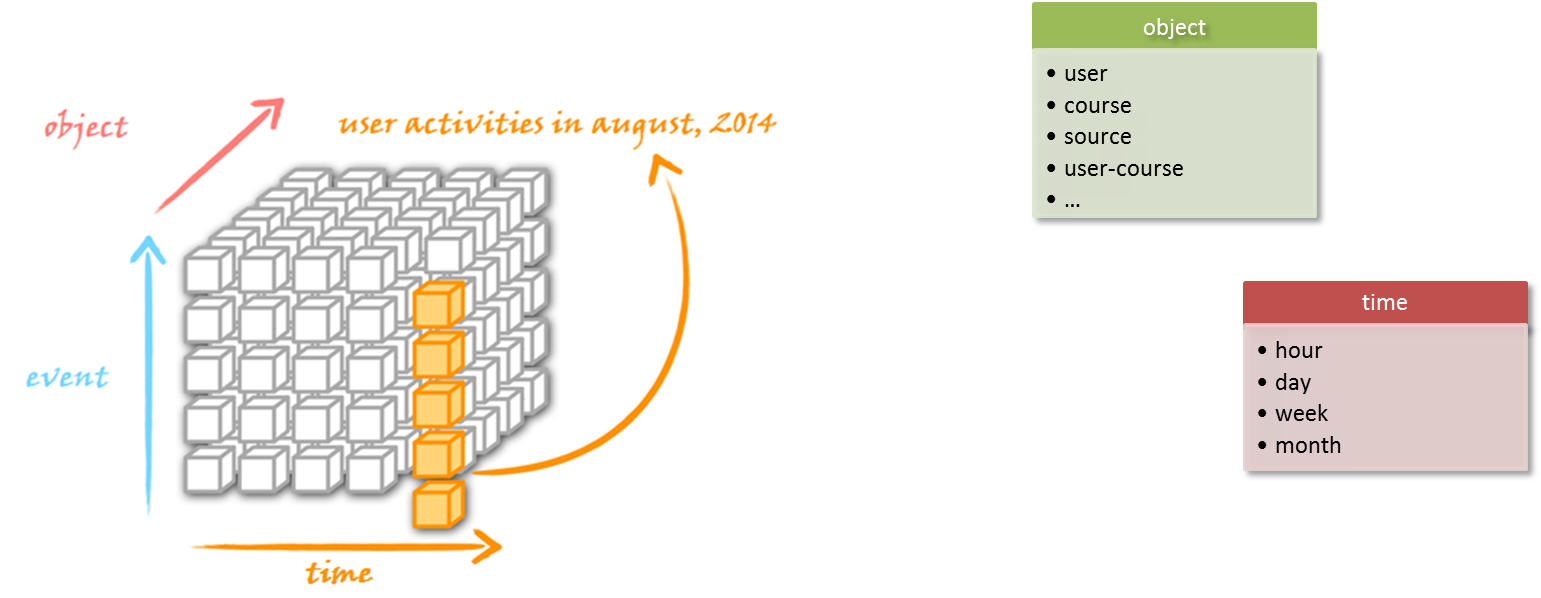
\includegraphics[width=1 \textwidth]{cube}
	\label{fig:cube}
\end{figure*}


\subsection{Common Features}
There are common features across 7 feature sets as follows:
\begin{itemize}
	\item Number of objects
	\item Number of events
	\item Aggregation features these count features
\end{itemize}
The common features can be generated using cube operations. Figure~\ref{fig:slice} shows an example how weekly and monthly count features are calculated. Firstly, the data is cut using object dimension. In this case, we choose to generate feature for users. Next, we select an event "navigate" in the event space to generate a time series presenting "navigate" event over the time. Finally, drill down operation is used to generate monthly or weekly count features.

\begin{figure*}[!t]
	\caption{Slice and Dice}
	\centering
	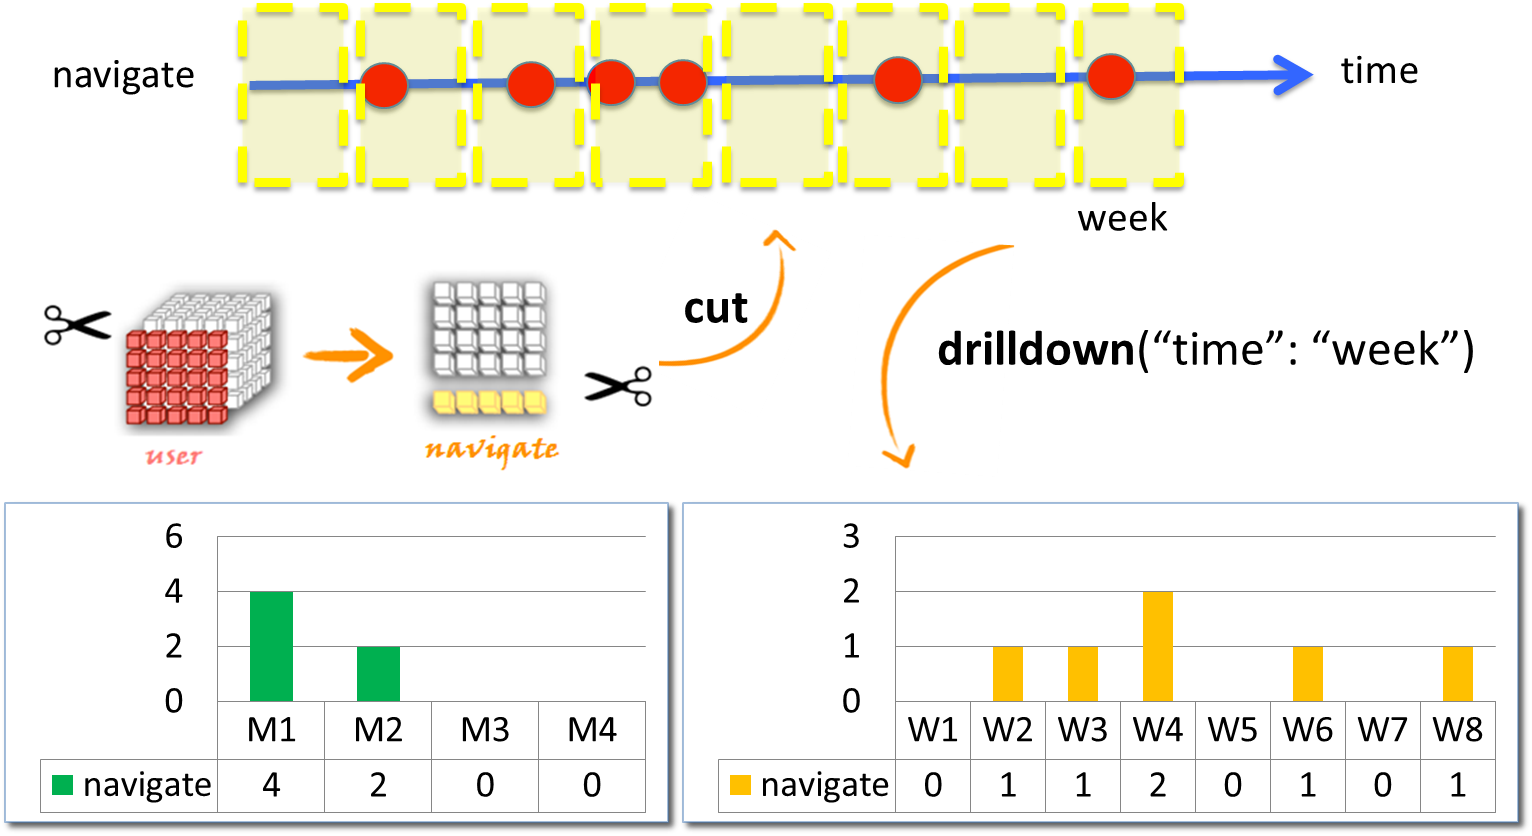
\includegraphics[width=1 \textwidth]{slice_and_dice}
	\label{fig:slice}
\end{figure*}

\subsection{F1}

Features generated by Song and Kohei can be classified as follows:

\begin{itemize}
  \setlength\itemsep{0em}
  \item Enrollment-based features (No.1-8)
  \item Username-based features (No.9-18)
  \item Username-based features for each courses (No.19-25) 
  \item Features based on 10 days after the end date of course (No.26-35)
  \item Features based on 1 day after the end date of a course (No.36-45)
  \item Day-level features (No.46)
  \item Day-level features using target variables (No.47-58)
\end{itemize}

Full list of features generated by Song and Kohei are described in Table~\ref{tb:skfeature}.
(just listing them for now. TBD in detail).

\begin{center}
  \begin{table*}[ht]
    \begin{minipage}{\textwidth}
    {
      \small
      \hfill{}
      \begin{tabular}{|l|l|}
      \hline
      \textbf{No.}&\textbf{Description}\tabularnewline \hline
      1 & Course\_id encoded by 1-of-N coding \tabularnewline
      2 & Number of requests by an enrollment\_id \tabularnewline
      3 & Number of unique object by an enrollment\_id \tabularnewline
      4 & Number of unique problem object of event by an enrollment\_id \tabularnewline
      5 & Number of active days by an enrollment\_id \tabularnewline
      6 & Number of active hours by an enrollment\_id \tabularnewline
      7 & Time of first access in hours by an enrollment\_id \tabularnewline
      8 & Time of last access in hours by an enrollment\_id \tabularnewline
      9 & Number of enrollments by an username \tabularnewline
      10 & Number of requests by an username \tabularnewline
      11 & Number of unique objects by an username \tabularnewline
      12 & Number of unique problem object of event by an username \tabularnewline
      13 & Number of active days by an username \tabularnewline
      14 & Number of active hours by an username \tabularnewline
      15 & Time of first access in hours by an username \tabularnewline
      16 & Time of last access in hours by an username \tabularnewline
      17 & Time of first problem access in hours by an username \tabularnewline
      18 & Time of last problem access in hours by an username \tabularnewline
      19 & For each course, number of requests by an username \tabularnewline
      20 & For each course, number of unique object by an username \tabularnewline
      21 & For each course, number of unique problem object by an username \tabularnewline
      22 & For each course, number of active days by an username \tabularnewline
      23 & For each course, number of active hours by an username \tabularnewline
      24 & For each course, time of first access in hours \tabularnewline
      25 & For each course, time of last access in hours \tabularnewline
      26 & Number of enrollment\_ids during 10 days after the end date of course by an username \tabularnewline
      27 & For each course, number of access logs during 10 days after the end date of course by an username \tabularnewline
      28 & For each course, number of unique objects during 10 days after the end date of course by an username \tabularnewline
      29 & For each course, number of unique problem objects during 10 days after the end date of course by an username \tabularnewline
      30 & For each course, number of active hours during 10 days after the end date of course by an username \tabularnewline
      31 & For each course, difference between first and last access during 10 days after the end date of course by an username \tabularnewline
      32 & For each course, time of first access in hours during 10 days after the end date of course by an username \tabularnewline
      33 & For each course, time of last access in hours during 10 days after the end date of course by an username \tabularnewline
      34 & For each course, time of first access to an problem object in hours during 10 days after the end date of course by an username \tabularnewline
      35 & For each course, time of last access to an problem object in hours during 10 days after the end date of course by an username \tabularnewline
      36 & Number of enrollment\_ids during 1 day after the end date of course by an username \tabularnewline
      37 & For each course, number of access logs during 1 day after the end date of course by an username \tabularnewline
      38 & For each course, number of unique objects during 1 day after the end date of course by an username \tabularnewline
      39 & For each course, number of unique problem objects during 1 day after the end date of course by an username \tabularnewline
      40 & For each course, number of active hours during 1 day after the end date of course by an username \tabularnewline
      41 & For each course, difference between first and last access during 1 day after the end date of course by an username \tabularnewline
      42 & For each course, time of first access in hours during 1 day after the end date of course by an username \tabularnewline
      43 & For each course, time of last access in hours during 1 day after the end date of course by an username \tabularnewline
      44 & For each course, time of first access to an problem object in hours during 1 day after the end date of course by an username \tabularnewline
      45 & For each course, time of last access to an problem object in hours during 1 day after the end date of course by an username \tabularnewline
      46 & For each days of the course, which date is provided in date.csv, number of unique active courses by an username \tabularnewline
      \hline
      \end{tabular}
    }
    \hfill{}
    \caption{List of features generated by Song and Kohei.}
    \label{tb:skfeature}
    \end{minipage}
  \end{table*}
\end{center}

\subsection{F2}
Peng and Xiaocong features are comprised of the following parts:
\begin{itemize}
  \setlength\itemsep{0em}
  \item Visit time(hour, day) set features (including time span and max absent days)
  \item Act(event, object) counting features (some uses missed content counts)
  \item Course drop rate
  \item Number of courses the user enrolled
  \item Minimum time interval between time points(first visit, last visit, course begin, course end, 10 days after course end) of current course and another enrolled course
  \item Active days between course end and 10 days after course end
  \item Active days between last visit and course end
  \item Number of courses ended after current course end
\end{itemize}

The full feature list could be found in Table~\ref{tb:rwfeature}.

\begin{center}
  \begin{table*}[ht]
    \begin{minipage}{\textwidth}
    {
      \small
      \hfill{}
      \begin{tabular}{|l|l|}
      \hline
      \textbf{No.}&\textbf{Description}\tabularnewline \hline
1 & act counts \tabularnewline
2 & hourset length in last 2 days \tabularnewline
3 & last month \tabularnewline
4 & max absent days \tabularnewline
5 & day set length \tabularnewline
6 & hour set length \tabularnewline
7 & average hours per day \tabularnewline
8 & event wiki counts \tabularnewline
9 & event discussion counts \tabularnewline
10 & event access counts \tabularnewline
11 & event video counts \tabularnewline
12 & event problem counts \tabularnewline
13 & obj chapter not visited \tabularnewline
14 & obj chapter visited ratio \tabularnewline
15 & obj video not visited \tabularnewline
16 & obj video visited ratio \tabularnewline
17 & obj problem not visited \tabularnewline
18 & obj problem visited ratio \tabularnewline
19 & obj set length \tabularnewline
20 & total time span \tabularnewline
21 & days from last act to course end \tabularnewline
22 & course drop rate \tabularnewline
23 & number of courses enrolled \tabularnewline
24 & min days between first visit and next course begin \tabularnewline
25 & min days between 10 days after last visit and next course begin \tabularnewline
26 & min days between last visit and next course end \tabularnewline
27 & min days between previous course end and last visit \tabularnewline
28 & min days between 10 days after current course end and next course begin \tabularnewline
29 & min days between 10 days after current course end and next course end \tabularnewline
30 & min days between current course end and next visit \tabularnewline
31 & number of active days between last visit and course end \tabularnewline
32 & number of active days in 10 days after course end \tabularnewline
33 & number of courses ended after current course end \tabularnewline
      \hline
      \end{tabular}
    }
    \hfill{}
    \caption{List of features generated by Peng and Xiaocong.}
    \label{tb:rwfeature}
    \end{minipage}
  \end{table*}
\end{center}

\subsection{F3}
These features were generated by Tam. They can be categorized into three major groups, count, aggregation, and date features. The list of features is as follows:
\subsubsection{Count Feature}
There are a few entities such as user, course, and object in the training dataset. Combining these entities together, we have user activities or events. The simplest way to generate features from these events is to count the number of times an entity engaging in the event. The motivation is that the more does a user participate in course, the more chance does he drop out that course. The list of count features are given in Table~\ref{tb:tnfeature1}.

\begin{center}
	\begin{table*}[ht]
		\begin{minipage}{\textwidth}
			{
				\small
				\hfill{}
				\begin{tabular}{|l|l|l|}
					\hline
					\textbf{No.}&\textbf{Feature}&\textbf{Description}\tabularnewline \hline
					1 & User counts & The log count of each user \tabularnewline
					2 & Course count & The log count of each course \tabularnewline
					3 & Event count & The log count of each event \tabularnewline
					4 & User weekly count & The log count of each user per week \tabularnewline
					5 & User bi-weekly count & The log count of each user per two weeks \tabularnewline
					6 & User weekday count & The log count of each user per weekday \tabularnewline
					7 & User monthly count & The log count of each user per month\tabularnewline
					8 & Course weekly count & The log count of each course per week \tabularnewline
					9 & Course bi-weekly count & The log count of each course per two weeks \tabularnewline
					10 & Course weekday count & The log count of each course per weekday\tabularnewline
					11 & Course monthly count & The log count of each course per month \tabularnewline
					12 & Event weekly count & The log count of each event per week \tabularnewline
					13 & Event bi-weekly count & The log count of each event per two weeks \tabularnewline
					14 & Event weekday count & The log count of each event per weekday \tabularnewline
					15 & Event monthly count & The log count of each event per month \tabularnewline
					\hline
				\end{tabular}
			}
			\hfill{}
			\caption{List of count features generated by Tam.}
			\label{tb:tnfeature1}
		\end{minipage}
	\end{table*}
\end{center}

\subsubsection{Aggregation Feature}
Aggregation features were calculated based on count features. Usually, each course would have a fixed schedule for users to study. Therefore, students roll in the course must have stable activity patterns. Aggregation features would measure the stability of course engagement. These features are mean, median, standard deviation of count on date basis such as weekly, monthly, etc. The list of aggregation features are given in Table~\ref{tb:tnfeature2}.

\begin{center}
	\begin{table*}[ht]
		\begin{minipage}{\textwidth}
			{
				\small
				\hfill{}
				\begin{tabular}{|l|l|l|}
					\hline
					\textbf{No.}&\textbf{Feature}&\textbf{Description}\tabularnewline \hline
					1 & Min & Min of all above count features \tabularnewline
					2 & Max & Max of all above count features \tabularnewline
					3 & Mean & Mean of all above count features \tabularnewline
					4 & Median & Median of all above count features \tabularnewline
					5 & Std & Standard deviation of all above count features  \tabularnewline
					\hline
				\end{tabular}
			}
			\hfill{}
			\caption{List of aggregation features generated by Tam.}
			\label{tb:tnfeature2}
		\end{minipage}
	\end{table*}
\end{center}

\subsubsection{Date Feature}
To capture how often users participate in a certain course, we generated date features. Date features can be time span among user activities as well as time span from last activity and last course date. The list of date features is given in Table~\ref{tb:tnfeature3}.

\begin{center}
	\begin{table*}[ht]
		\begin{minipage}{\textwidth}
			{
				\small
				\hfill{}
				\begin{tabular}{|l|l|l|}
					\hline
					\textbf{No.}&\textbf{Feature}&\textbf{Description}\tabularnewline \hline
					1 & Min time span & Min time span among activities \tabularnewline
					2 & Max time span & Max time span among activities \tabularnewline
					3 & Mean time span & Mean time span among activities \tabularnewline
					4 & Last time span & Time span from the last activity and last course date \tabularnewline
					5 & Number of unique days & The number of unique activity days of each user \tabularnewline
					\hline
				\end{tabular}
			}
			\hfill{}
			\caption{List of date features generated by Tam.}
			\label{tb:tnfeature3}
		\end{minipage}
	\end{table*}
\end{center}

\subsection{F4}
Features generated by Michael Jahrer are in sparse format:

\begin{itemize}
  \setlength\itemsep{0em}
  \item uID (0-112,447)
  \item cID (112,448-112,486)
  \item uIDcnt (112,487-112,487)
  \item eIDcnt (112,488-112,488)
  \item eID $\rightarrow$ sID (112,489-112,490)
  \item eID $\rightarrow$ evID (11,2491-112,497)
  \item eID $\rightarrow$ oIDCnt (112,498-139,443)
  \item eID $\rightarrow$ tIDCnt (139,444-139,635)
  \item uID: floor(log(dateSpan$^2$+1)) (139,636-140,635)
  \item uID $\rightarrow$ log(time diff to obj start+1) (140,636-140,636)
  \item eID $\rightarrow$ dateVec diff stats (140,637-140,649)
\end{itemize}

\subsection{F5}
\begin{itemize}
  \setlength\itemsep{0em}
  \item Course ID - One-hot-encoded course\_id
  \item Source time counts  by enrollment - The log count of each source type per day for each enrollment
  \item Source time counts by course id - The log count of each source type per day for each course id
  \item Event time counts by enrollment - The log count of each event type per day for each enrollment
  \item Event time counts by course id - The log count of each event type per day for each course id

\end{itemize}

\subsection{F6}
Features generated by Jeong-Yoon Lee are as follows:

\begin{itemize}
  \setlength\itemsep{0em}
  \item User ID (20,113) - One-hot-encoded username. Usernames appearing less than 100 times in training log data are grouped together as one user ID. 
  \item Course ID (39) - One-hot-encoded course\_id.
  \item Source Event (10) - One-hot-encoded combination of source and event.
  \item Object ID (3,554) - One-hot-encoded object.  Objects appearing less than 100 times in training log data are grouped together as one object ID.
  \item Count (1) - Number of log entries for an hour\_id.
  \item Object Category (6) - Number of log entries with an object category for an enrollment\_id.
  \item Number of Children Objects (7) - One-hot-encoded total number of object's children for an enrollment\_id.
  \item Object Timespan (10) - One-hot-encoded timespan in days between object's start date and last day of the class
  \item Day of Class (30) - One-hot-encoded day of the class
  \item Week of Class (4) - One-hot-encoded week of the class
  \item End Month of Class (7) - One-hot-encoded end month of the class
  \item Object Started in Dropout Period (2) - Binary variable that is 1 if object started after but before 10 days after last day of the class and 0 otherwise.
\end{itemize}

\subsection{F7}

F1 features and additional features generated by Kohei. Additional features are as follows:

\begin{center}
  \begin{table*}[ht]
    \begin{minipage}{\textwidth}
    {
      \small
      \hfill{}
      \begin{tabular}{|l|l|}
      \hline
      \textbf{No.}&\textbf{Description}\tabularnewline \hline
      1 & For each 10 days after the end date of the course, number of active enrollment\_id, which target variables are 1 in the training set, enrolled by an username \tabularnewline 
      2 & For each 10 days after the end date of the course, number of active enrollment\_id, which target variables are 0 in the training set, enrolled by an username \tabularnewline 
      3 & For each 10 days after the end date of the course, number of active enrollment\_id (in this case, days between last access and the end date of the course are also counted for active days), which target variables are 1 in the training set, enrolled by an username \tabularnewline
      4 & For each 10 days after the end date of the course, number of active enrollment\_id (in this case, days between last access and the end date of the course are also counted for active days), which target variables are 0 in the training set, enrolled by an username \tabularnewline
      5 & For each 14 days before the end date of the coruses, number of active enrollment\_id, which target variables are 1 in the training set, enrolled by an username \tabularnewline 
      6 & For each 14 days before the end date of the coruses, number of active enrollment\_id, which target variables are 0 in the training set, enrolled by an username \tabularnewline 
      7 & For each 14 days before the end date of the coruses, number of active enrollment\_id (in this case, days between last access and the end date of the course are also counted for active days), which target variables are 1 in the training set, enrolled by an username \tabularnewline
      8 & For each 14 days before the end date of the coruses, number of active enrollment\_id (in this case, days between last access and the end date of the course are also counted for active days), which target variables are 0 in the training set, enrolled by an username \tabularnewline
      \hline
      \end{tabular}
    }
    \hfill{}
    \caption{List of additional features generated by Kohei.}
    \label{tb:skfeature}
    \end{minipage}
  \end{table*}
\end{center}

\section{Classification Algorithms}
We selected algorithms that achieve good predictive performance, process large sparse data sets efficiently (with exception of K-Nearest Neighbors) and differ from other algorithms.  The 8 classification algorithms selected are as follows:
\begin{itemize}
\setlength\itemsep{0em}
\item \textbf{Gradient Boosting Machine (GBM)}: We trained GBM classifiers using the Scikit-Learn Python package \cite{scikit-learn} and XGBoost \cite{chen2015xgboost}.  We used various tree structures of 4 to 10 maximum depths and 0.004 to 0.05 shrinkage rates.
\item \textbf{Neural Networks (NN)}: We trained NN classifiers with the dropout \cite{srivastava2014dropout}, ReLU transfer function and sigmoid activation function.  We used various network architectures of 1 to 3 hidden layers and 16 to 500 hidden units per layer.  We wrote our own C++ NN implementation optimized for sparse data sets.  
\item \textbf{Factorization Machine (FM)}: We trained FM classifiers using libFM \cite{rendle2012factorization} and libFFM \cite{libffm}.  We used 2-way interaction dimensions of 4 to 20.  We transformed count variables $x$ into $\log{(1 + x)}$.
\item \textbf{Logistic Regression (LR)}: We trained LR classifiers using the Scikit-Learn Python package \cite{scikit-learn} and Vowpal Wabbit \cite{langford2007vowpal}.  We used the regularization parameter $C=0.01$.  We transformed count variables $x$ into $\log{(1 + x)}$.
\item \textbf{Kernel Ridge Regression (KRR)}: We trained KRR classifiers using our own C++ implementation.  We used the ridge regression constant $\lambda=1.5e-3$ with the Gaussian kernel.  We transformed count variables $x$ into $\log{(1 + x)}$.
\item \textbf{Extremely Randomized Trees (ET)}: We trained ET classifiers using the Scikit-Learn Python package \cite{scikit-learn}.
\item \textbf{Random Forests (RF)}: We trained RF classifiers using the Scikit-Learn Python package \cite{scikit-learn}.  Besides training classifiers, we used RF for feature selection.  We trained an RF model and selected features with high variable importances.
\item \textbf{K-Nearest Neighbors (KNN)}: We trained KNN classifiers using our own C++ implementation.  We used $k=124$ with the Euclidean distance.  We transformed count variables $x$ into $\log{(1 + x)}$.
\end{itemize}
\section{Learning Framework}
At previous KDD Cups, winning solutions either combined only single models without further combining ensemble models \cite{guyon2009analysis, yu2010feature} or combined ensemble models based on public leaderboard scores, which are not available in practice \cite{chen2011, wu2012two}.

However, we were able to combine ensemble models in multiple stages without overfitting to training data or using public leaderboard scores by using our learning framework.  Our learning framework consists of the stratified cross validation (CV) and multi-stage ensemble.

\subsection{Model Validation}

\begin{figure}
  \centering
    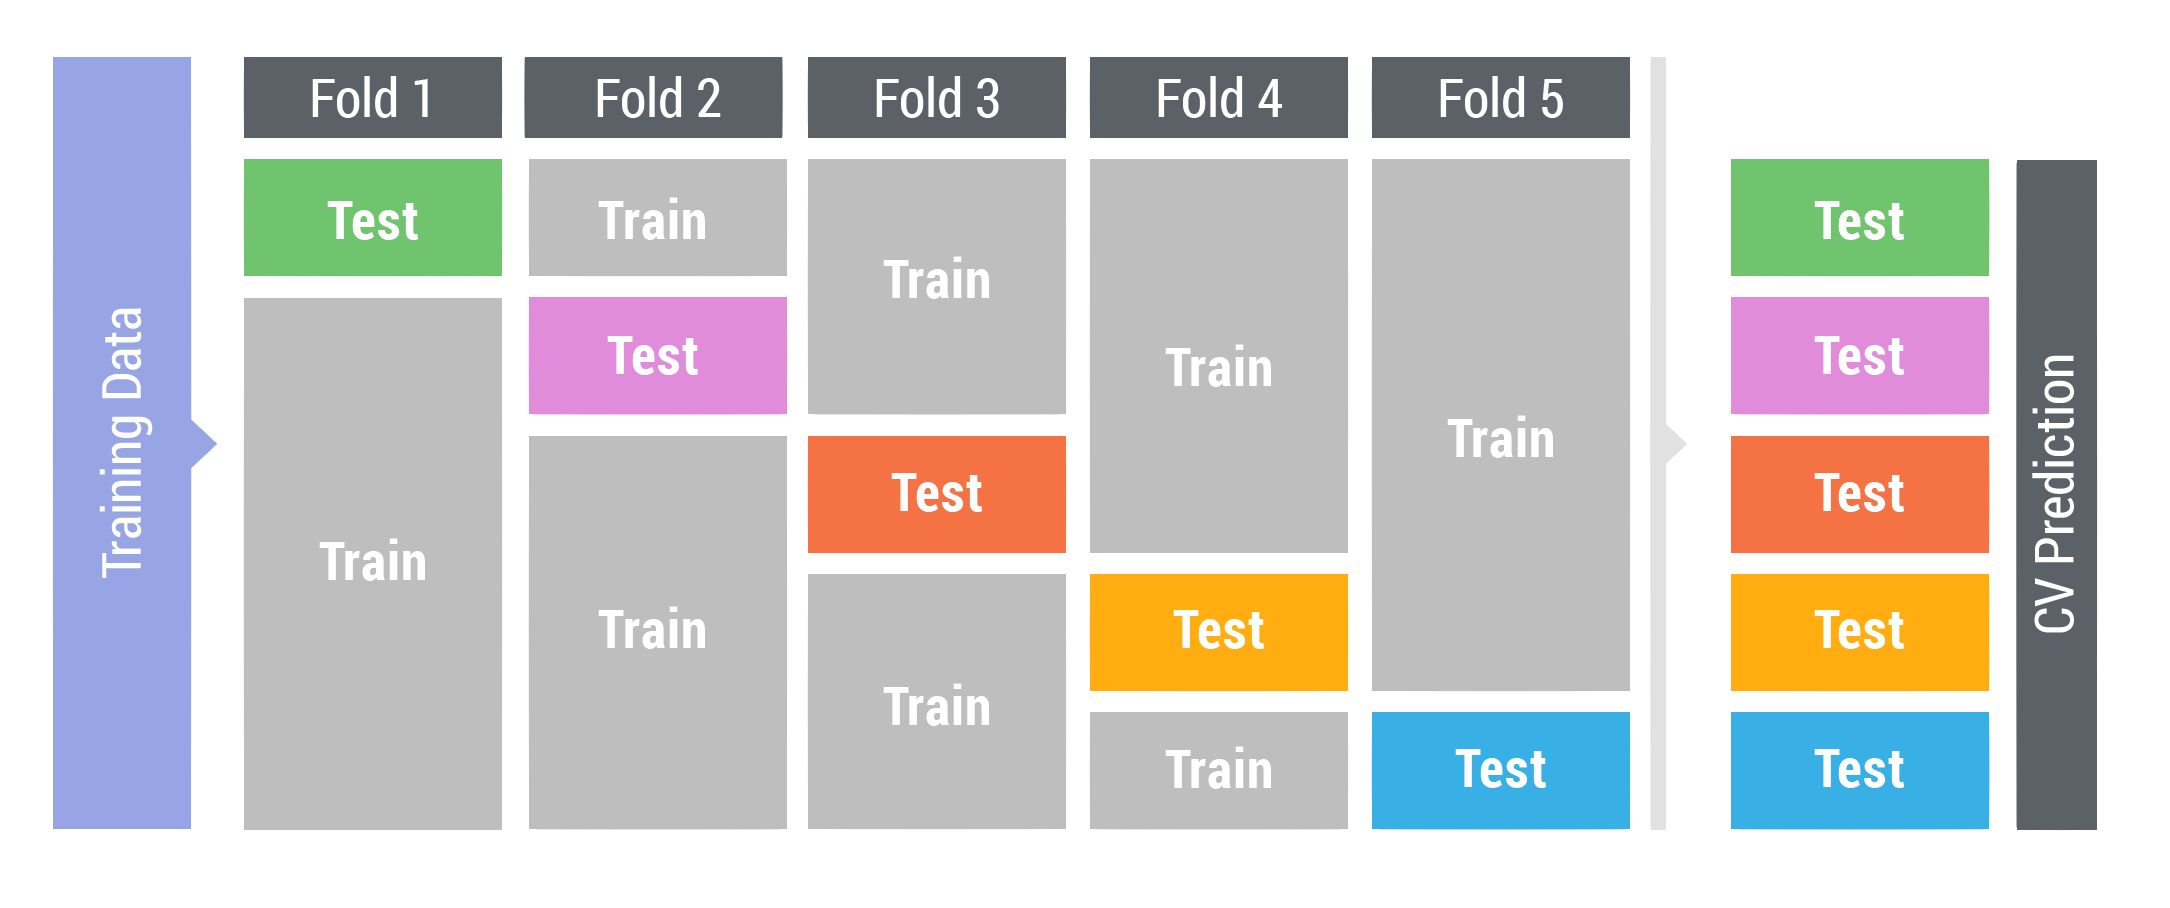
\includegraphics[width=0.5 \textwidth]{cv}
    \caption{5-fold CV.}
\end{figure}

We used stratified 5-fold CV for model validation and ensemble.
As shown in Figure 3, training data were split into 5 folds while the sample size and dropout rate were preserved across the folds.

For validation, each of single and ensemble models was trained 5 times. Each time, 1 fold was held out and the remaining 5 folds were used for training. Then, predictions for the hold-out folds were combined and formed the model's CV prediction. CV predictions were used as inputs for ensemble model training as well as the model's CV score calculation.

For test, each of single and ensemble models was retrained with whole training data. Then predictions for test data were used as inputs for ensemble prediction as well as for submission. 

\subsection{Multi-Stage Ensemble}

\begin{figure}[!h]
  \centering
    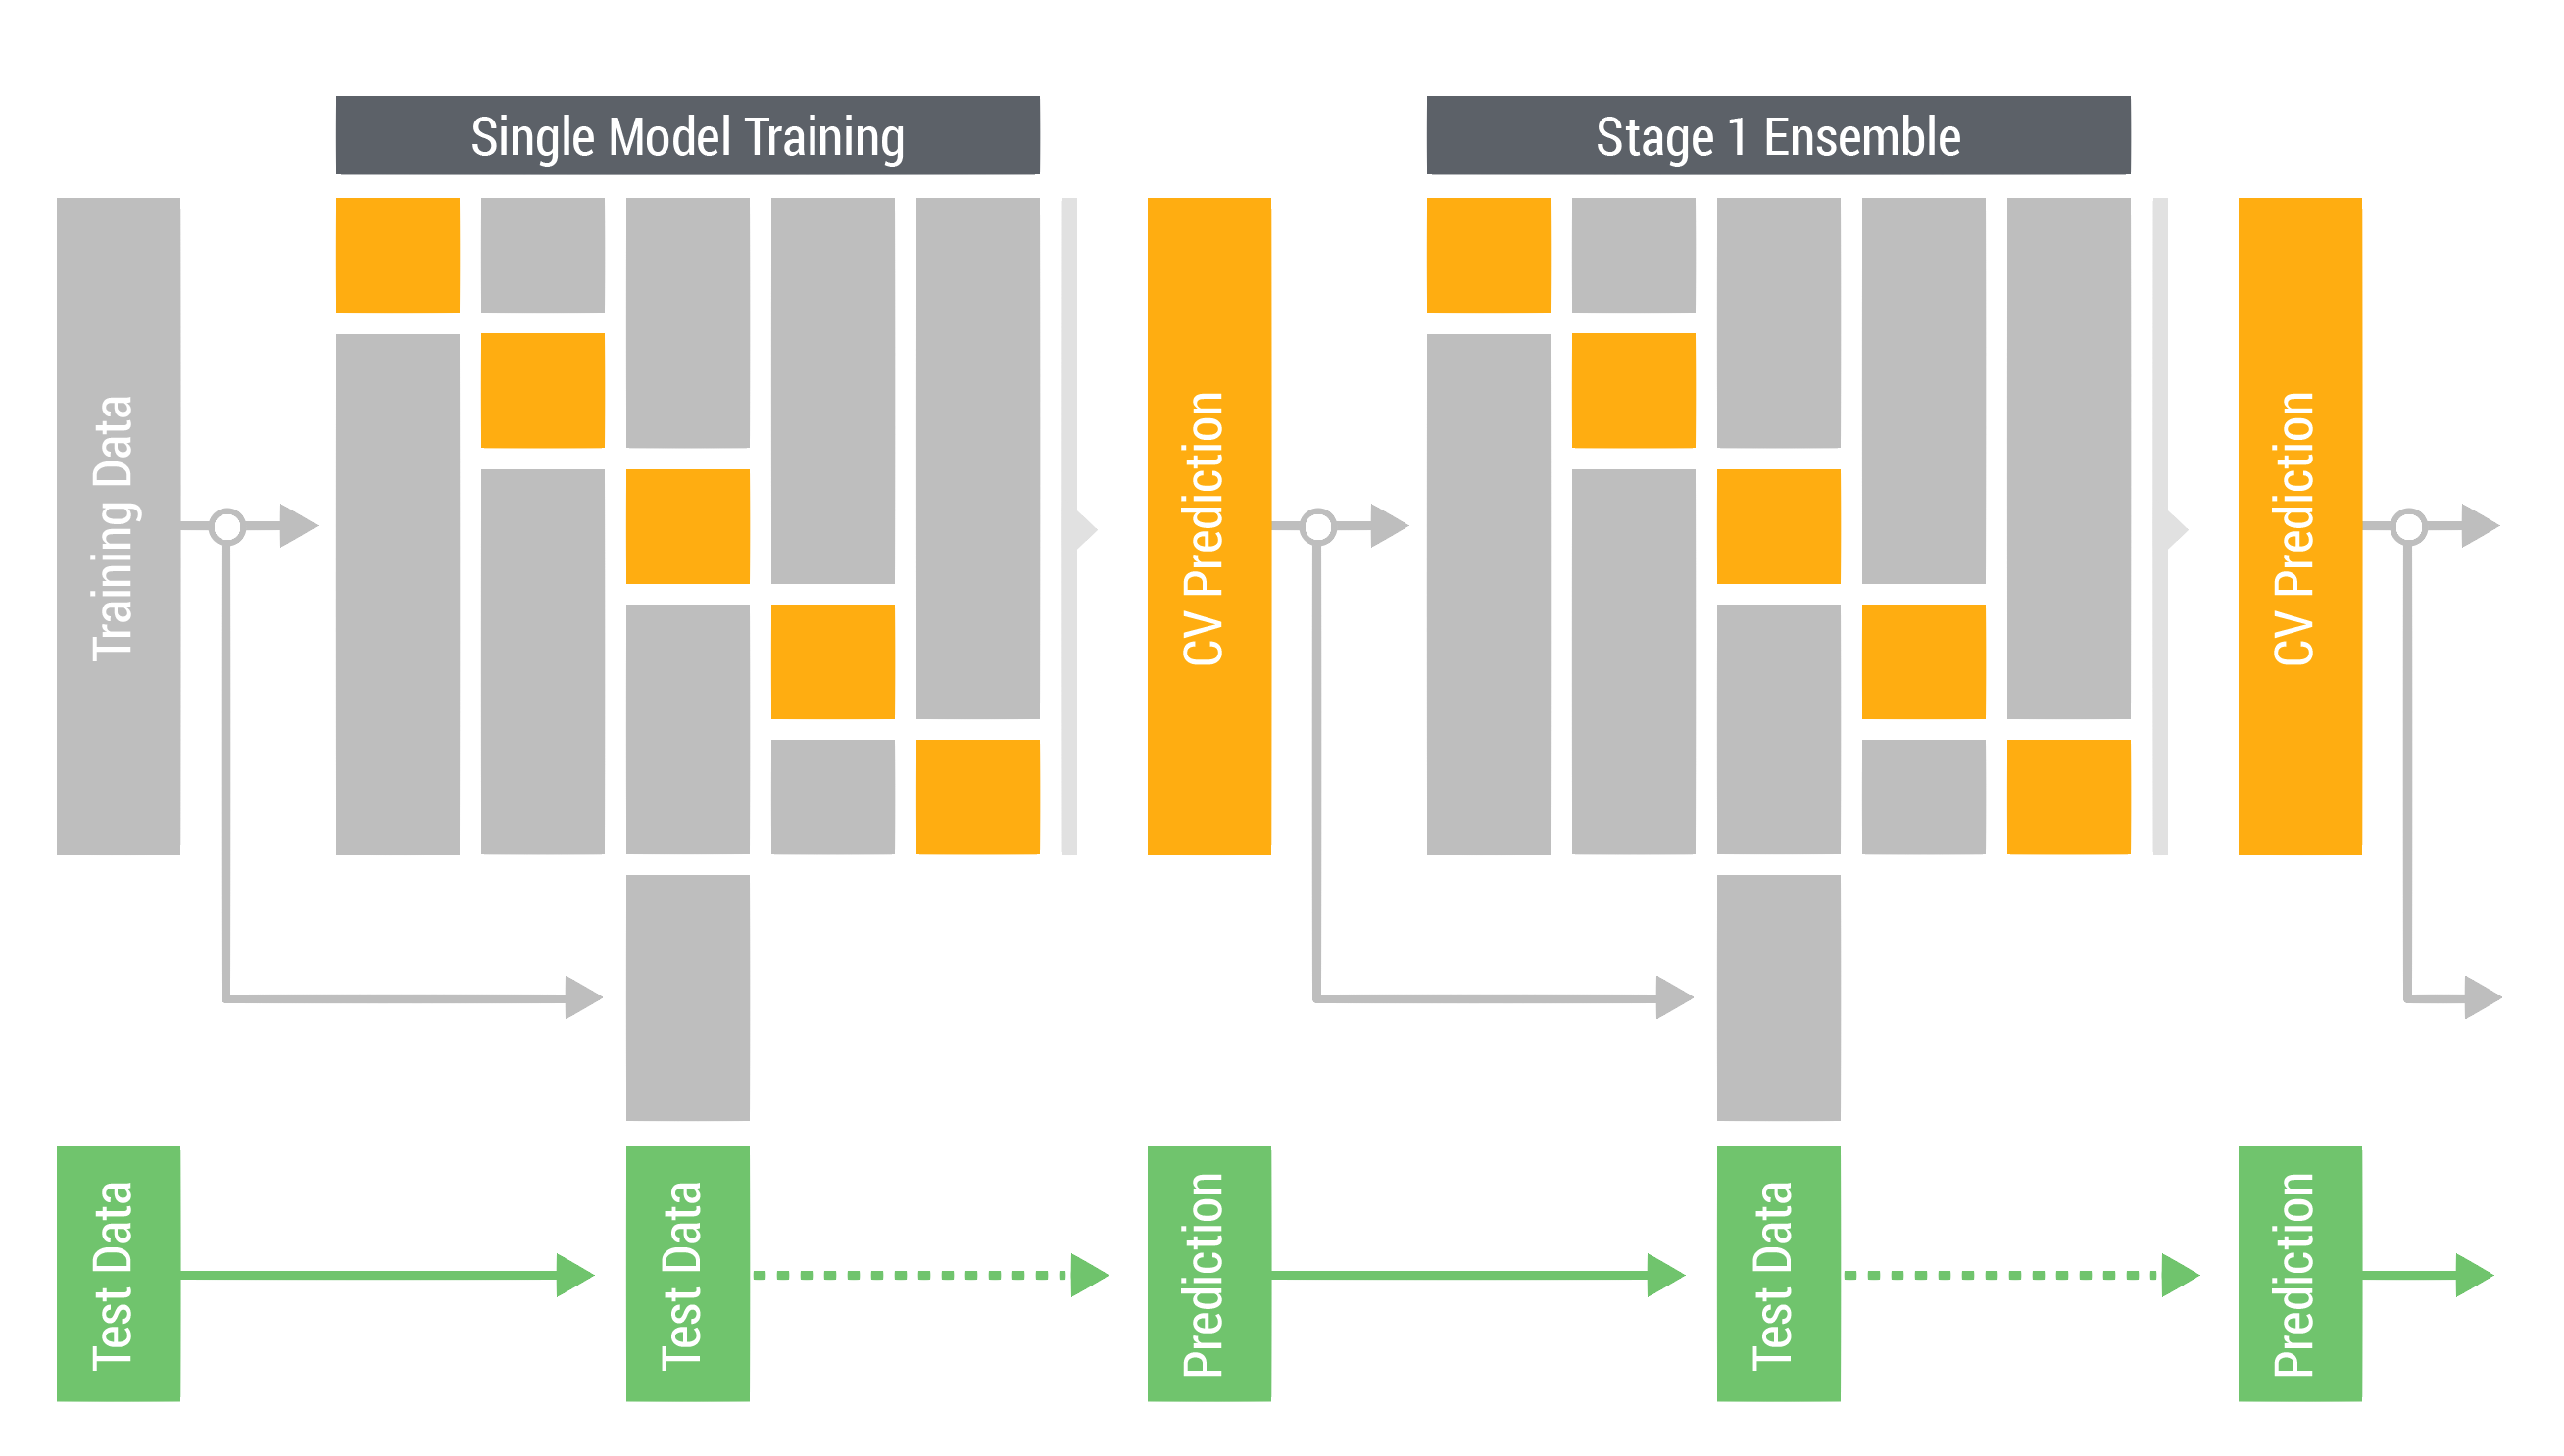
\includegraphics[width=0.5 \textwidth]{cv_ensemble}
      \caption{5-fold CV stacked generalization ensemble.}
\end{figure}

We used the multi-stage ensemble with stacked generalization \cite{wolpert1992stacked, ting1999issues} to blend predictions of various models.  At each stage, we train ensemble models with 5-fold CV, and use the CV and test predictions of models in the previous stage as inputs.  Then, we pass the CV and test predictions of the ensemble models to the next stage as inputs.  Figure 4 illustrates the process of multi-stage ensemble with 5-fold CV stacked generalization.

We stopped adding an additional ensemble stage when we saw no improvement in CV.
\section{Final Solution}
Our final solution is a stage-3 ensemble model trained with the multi-stage ensemble method described in Section 4.2 as follows:
\begin{itemize}
  \setlength\itemsep{0em}
  \item \textbf{Single Model Training}: First, we trained 64 single models with the 8 different algorithms and different subsets of 7 feature sets and DAE features.  Out of 64 models, there were 26 GBM, 14 NN, 12 FM, 6 LR, 2 KRR, 2 ET, 1 RF, and 1 KNN models.  Some of single models used RF feature selection, where we trained an RF model and selected features with high variable importances.
  \item \textbf{Stage-1 Ensemble}: Second, we trained 15 stage-1 ensemble models with different subsets of CV predictions of 64 single models.  Out of 15 models, there were 7 GBM, 4 NN, 2 LR, 1 FM, and 1 ET models.  Some of stage-1 ensemble models used rank orders between single models as additional inputs.  
  \item \textbf{Stage-2 Ensemble}: Third, we trained 2 stage-1 ensemble models with different subsets of CV predictions of 15 stage-1 ensemble models.  We used a LR with stepwise greedy forward selection and a GBM.
  \item \textbf{Stage-3 Ensemble}: Lastly, we trained a stage-3 ensemble model with CV predictions of all models.  We used LR with stepwise greedy forward selection, and it selected 5 models out of total 81 models: 1 stage-2 ensemble models, 3 stage-1 ensemble models and 1 single model.  Table 3 shows the list of models selected by the final stage-3 ensemble model.
\end{itemize}

Figure 6 shows the end-to-end pipeline for the final solution.  Details of the single and ensemble models trained are available in Table A3 and A4 in Appendix.

Our final solution achieved AUC scores of 0.90918 and 0.90744 on the public and private leaderboards respectively, and put us to the 1st place out of 821 teams.

At KDD Cup 2015, we made some observations as follows:
\begin{itemize}
\setlength\itemsep{0em}
\item As shown in Figure 5, our CV scores were very consistent with public leaderboard scores.  Therefore we used CV scores to determine (1) whether to add more ensemble stage or not and (2) whether to include a model for ensemble or not.
\item GBM outperformed other algorithms.  Our top 8 single models as well as top 2 stage-1 ensemble models are GBM models.  NN and FM were next best algorithms.  LR with stepwise greedy forward selection worked well in ensemble stages.
\item Biggest performance improvement was from the stage-1 ensemble, and as we added more ensemble stages, we observed diminishing improvements.  The stage-1, -2, and -3 ensembles improved the best CV score by 0.00967, 0.00028, and 0.000226 respectively.  However, it was the improvement from the stage-2 and -3 ensemble that allowed us to finish the 1st.
\end{itemize}

\begin{figure}[t]
  \centering
    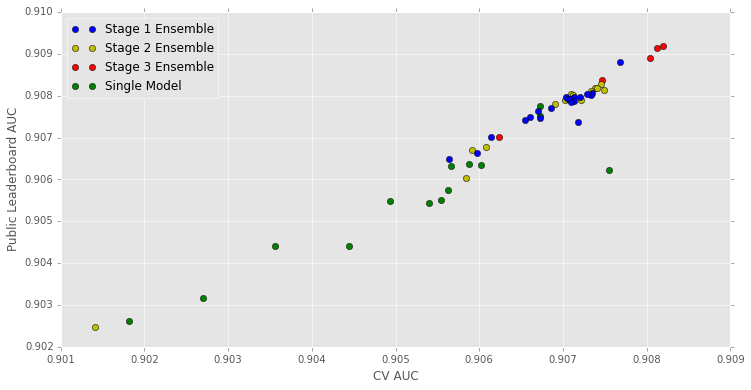
\includegraphics[width=0.5 \textwidth]{cv_lb}
      \caption{CV vs. public leaderboard AUC scores.}
\end{figure}

\begin{figure}[!t]
  \centering
    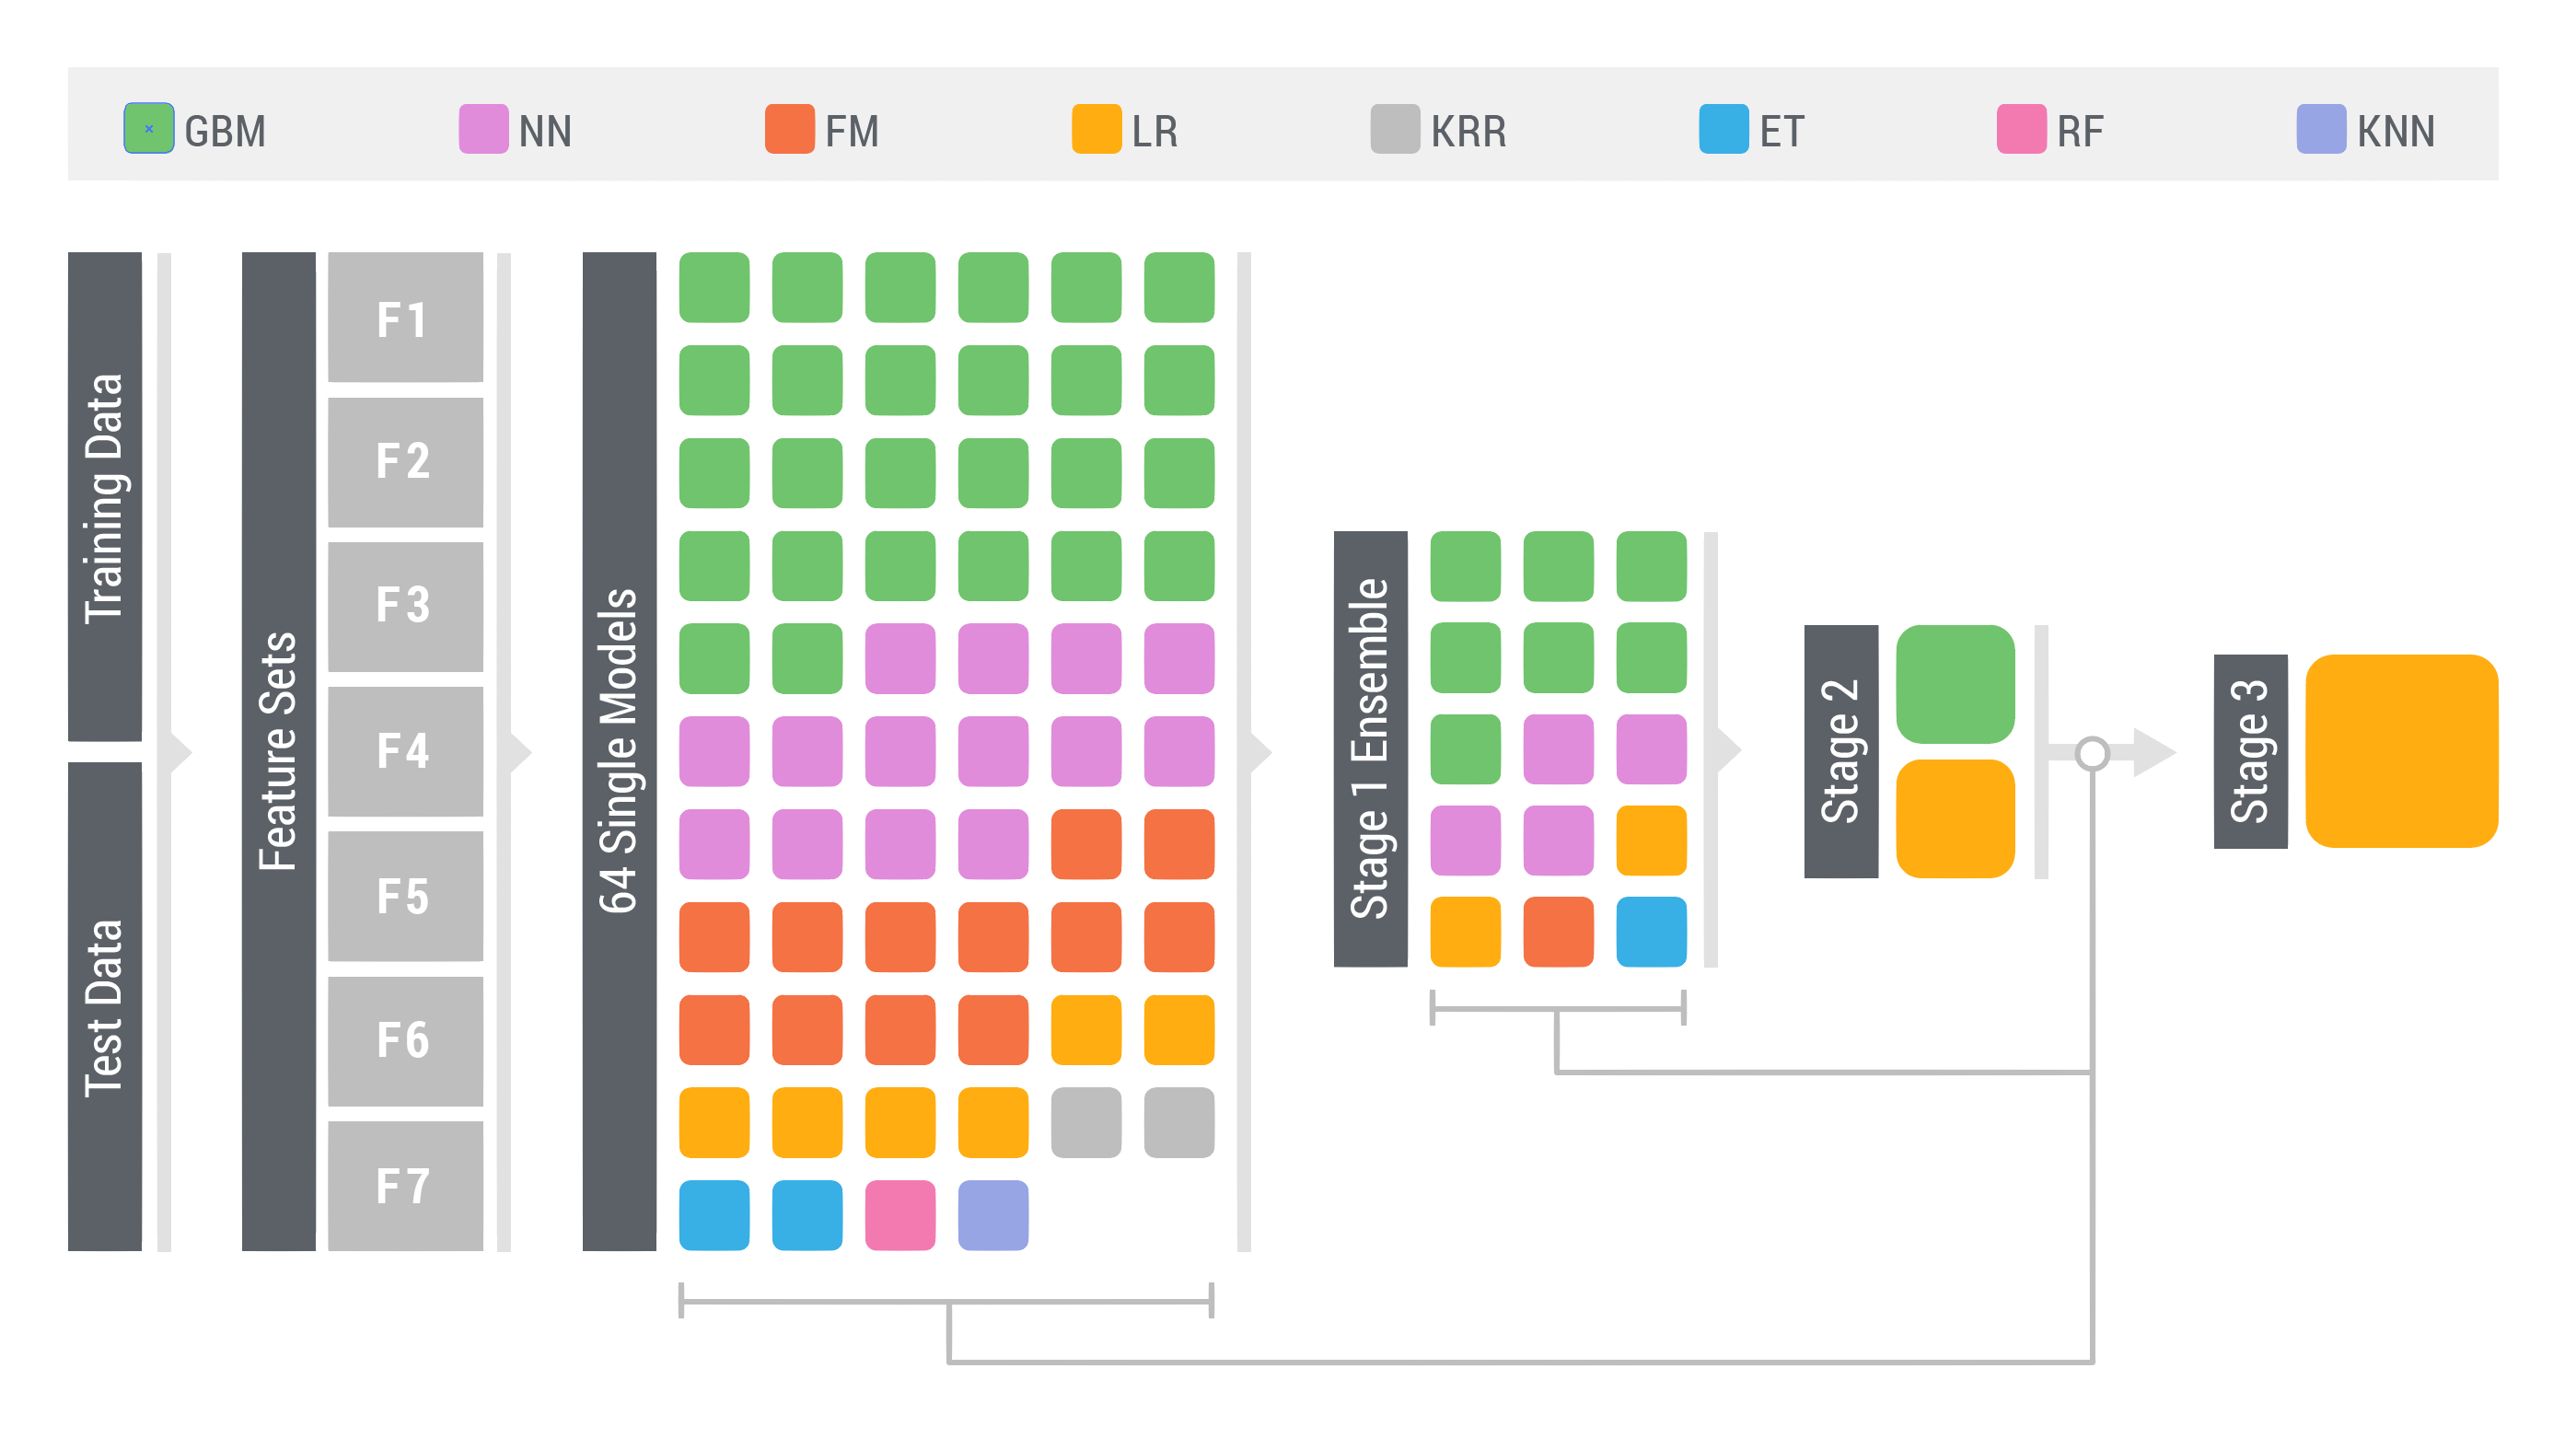
\includegraphics[width=0.5 \textwidth]{ensemble}
      \caption{End-to-end pipeline for the final solution}
\end{figure}

\begin{table}
\begin{center}
	\caption{Models selected in the stage-3 ensemble.}
\begin{tabular}{lllll}
ID 	& Stage 	& Algorithm 	& 5-CV 		& Weight\\ \hline
S1 	& Single	& GBM		& 0.906721 	& 1.1703 \\
E4 	& 1 		& GBM		& 0.907878 	& 1.9626\\
E8 	& 1 		& NN		& 0.907567	& 0.7871\\
E18	& 1		& ET			& 0.906207 	& 0.4580\\
E2	& 2 		& LR			& 0.907968 	& 1.6146\\
\end{tabular}

\label{tb:finalEnsemble}
\end{center}
\end{table}

\section{Conclusions}
Our final AUC score of 0.90918 results from a complex pipeline from raw data to final score.
Every part of that pipe needs to be (sub-)optimal implemented by our team to get the best score at the end.
The first part ``feature design'' is the most important one and needs expertise, experience and of course a bit luck to capture all signals in the data.

\bibliographystyle{abbrv}
\bibliography{sigproc}  % sigproc.bib is the name of the Bibliography in this case
% You must have a proper ".bib" file
%  and remember to run:
% latex bibtex latex latex
% to resolve all references
%
% ACM needs 'a single self-contained file'!

\end{document}
